Dans l'introduction de son livre ``Island Life'' paru en 1980 (soit 22
ans après la parution de \emph{On the Tendency of Varieties to Depart
Indefinitely From the Original Type}), le célèbre naturaliste Alfred
Russel Wallace saisit le drôle de paradoxe suivant : bien que séparé
traversé une bonne partie du globe terre les écosystème du Japon et du
Royaume Uni sont très similaire notamment par leur composition en
arbustes et en oiseaux alors que dans le même temps des êtres très
rapprochées comme les îles indinesiennes Bali et Lombok séparées de
quelques dizaines de kilomètres et peuvent être très différentes. Il
evoque aussi la faible predictibility du climat pour comprendre les
espèces en question , il prend pour exemple diff.érence faune afrique et
brésilienne malgès la similarité du climat. Face à ces paradoxes so
ouvrage ce veut une tentatatove pour comprendre ce les raisons mais il
reconnait dès l'introduction que :

\begin{quote}
Many years study of this class of subjects has convinced me that there
is no short abd easy method of dealing with them; because they are, in
their very nature, the visible outcome and residual product of the whole
past history of the earth.
\end{quote}

Dans une vision simplifiée l'écologie détermine les lien entre les
caractéristiques des espcèes de la mort et des naissance des et
l'évolution regardera les conséquences sur ces caractéristiques de ces
même morts et naissances. En prennant ces définitions on comprend
l'intrication de ces deux qui explique la demande pour réunir les deux
de même que diverse discipline on été réunie avec succès lors de la
théorie synthétique de l'évolution (Schoener, 2011).

porblème d'intricatoition des processus

Special attention sur les îles

Premier chapitre plus d'espèce mais plus de paramètre plus de porblème
moins de prédiction

Je vais illustrer mon propos avec 2 (3?) récurrent exemple (mais
d'autres aussi) le cas du Frelon asiqtieu (anglais : Yellow-legged
horne, \emph{Vespa velutina}). Importance pour impact dans sur les
abaeilles domestiques mais très peu sur la faune locale et les oiseaux
migrateurs dans le nord

L'introduction aux chapitres de ma thèse sera articulée autour de la
question fondamnetal esuivant

Dans cette introduction à ma thèse j'ai choisi de prendre comme fil
conducteur la question suivante : quelles informations referment la
distribution géographiques des espèces ? Pour y apporter un maximum
d'élément de réponse je regarderais les mécanismes sous-jacents à
l'échelle d'une échelle avant d'aborder les espoir que soulève l'analyse
de la variation de ces ranges dans le temps et l'espèce sur les
différentes échelles de temps avant d'aborder les apporter un maximum
d'é avant de montrer que l'analyse jointe semble révéler et les défis au
regard.

: question d'échelle / de variation de co-variation / difficultés
d'apprécier la proportions relative des différents mécanismes /
mécanismes de coexistence coexistence vs co-occurrence

variabilité quelle espoir de généralisation

Crombie repris dans Macarthur =\textgreater{} coexistence

Problème de coexistence

=\textgreater{}~non reproductibilité des ranges / stochasticité des
ranges Frelon asiatiques

=\textgreater{} degat sur la nouvelle faune local msiaune augmentation
++ du nombre de liens\ldots{} reconfigurations des réseaux locaux.

=\textgreater{} ou est le cuyrseur dans l'hstoire (evolution) ou la
geographie (l'ecologie)

A quel point est-il pertinent d'évaluer le range d'une espèce sur juste
une île.

Un problème d'identification.

classique experience de perte de la biodiv =\textgreater{} et hope une
histoire différenteds

raseemblé ecologie et Schoener (2011)

\section*{Section non num}\label{section-non-num}
\addcontentsline{toc}{section}{Section non num}

\section{Phase quantitavive /
modéliser}\label{phase-quantitavive-moduxe9liser}

\subsection{L'importance des îles en
biogéorgaphie}\label{limportance-des-uxeeles-en-bioguxe9orgaphie}

Décrire l'organisation spatiale des êtres vivants et en comprendre les
mécanismes sous-jacents, tels sont les objectifs ambitieux de la
biogéographie \cite{MacArthur1967}. Cette discipline a récemment
percolée au sein de la société civile via le concept de biodiversité. Le
regard des citoyens se posent attentivement sur le devenir de la
biodiversité dans le contexte actuel des changements globaux. La
biogéographie, par son essence, peut apporter des réponses à ce
questionnement ambiant \cite{Whittaker2005}. Cependant, pour y parvenir,
des défis techniques et théoriques majeurs restent à surmonter
\cite{Beck2012}.

L'effort théorique nécessaire en biogéographie porte sur l'intégration
ordonnée de concepts clés issus de différents champs de l'écologie
\cite{Thuiller2013}. Ainsi, alors que les conditions climatiques et plus
généralement la géographie physique sont classiquement évoquées pour
expliquer la répartition des espèces \cite{Kearney2004}, les
interactions entre espèces sont quant à elles souvent occultées. De
même, bien que les processus évolutifs soient souvent évoqués comme
déterminants majeurs de la diversité des espèces \cite{Rosindell2011},
leurs effets à court terme sont souvent ignorés \cite{Parmesan2006} dans
les scénarios décrivant la biodiversité de demain \cite{Lavergne2010}.
La difficulté principale est alors de produire des modèles (théoriques
en première instance) qui intègrent l'ensemble des processus et les
relations qu'ils entretient \cite{Thuiller2013} tout en gardant une
relative simplicité. Une théorie intégrative en biogéographie pourrait
être le meilleur point d'ancrage pour construire de nouvelles approches
appliquées. Avec une telle théorie en main, nous pourrions aller vers
l'enjeux majeurs de ces dernières années en biogéographie : relâcher les
hypothèses que les modèles classiques de répartitions des espèces
d'aujourd'hui utilisent (notamment en occultant les interactions) pour
prédire la biodiversité de demain \cite{Guisan2011}.

Dans le projet ici présenté, nous proposons de construire des modèles
théoriques plus intégratifs en repartant d'un modèle théorique
classique, celui de la théorie de la biogéographie des îles proposée par
MacArthur et Wilson \cite{MacArthur1967}. Dans un premier temps, nous y
ajoutons les interactions entre espèces et une relation explicite avec
l'environnement abiotique au travers d'une approche communauté centrée
qui étend le modèle classique. Dans un second temps, nous combinons une
approche population centrée et les processus évolutifs pour une
biogéographie insulaire plus mécaniste. Enfin, au regard des enjeux que
soulève le rôle des interactions entre espèces dans la construction de
la biodiversité, nous réfléchissons sur l'inférence d'espèces
interdépendantes.

\section{Data availability}\label{data-availability}

\section{Information dans les
distributions}\label{information-dans-les-distributions}

\subsection{Proxy}\label{proxy}

\subsection{Potential interactions}\label{potential-interactions}

Vespa aussi au Amérqieu la densit. des traffic\ldots{}

Multi couche de distrobution dans le cas du frelon asiatique Villemant
et al. ({\textbf{???}}) ont montrés que superposition du genre
\emph{Vespa} et notamment au niveau asiatique énormément aisin
l'inférence se fait sur des données qui comporte une empreinte de
condition et localemnt éteinte alors que possiblement comtraite qui ne
seront pas en France\ldots{}

\subsection{Enjeux essentiels de la
biogéographie}\label{enjeux-essentiels-de-la-bioguxe9ographie}

\subsection{Une question d'échelle}\label{une-question-duxe9chelle}

Question d'échelle La biogéographie avec au moins 3 problèmes d'échelles

=\textgreater{} spatiale peut-on avoir d

=\textgreater{} temporelle plus on augmente plus l'enpreinte historiques
est forte =\textgreater{} grands evenemnt géologique (lacitaion
mouvement des plques) biogéogrpahies historiqyes mais aussi forme un
pool d'espèces

=\textgreater{} Mais aussi l'échelle taxonomique : la relaton aire
espèce est décrite à l'intérieru des taxons les relations allométriques
à l'inérieur des taxons E O Wilson a commencé à rappporter des relation
sur les formis les exemples du livre sont herpeta faun (reptile plus
amphibien) mecanisme =\textgreater{} diversité de milieu

contre exemple des chauves souris

\section{Cadre théorique de la
thèse}\label{cadre-thuxe9orique-de-la-thuxe8se}

\subsection{Développements théoriques en
Biogéographie}\label{duxe9veloppements-thuxe9oriques-en-bioguxe9ographie}

equilibre =\textgreater{} equation 3-3 repartir de 3-3

\subsubsection{L'empreinte historique de la La Théorie de la
Biogéographie des Iles de MacArthur et
Wilson}\label{lempreinte-historique-de-la-la-thuxe9orie-de-la-bioguxe9ographie-des-iles-de-macarthur-et-wilson}

=\textgreater{} impact enorme sur la conservation et encore aujourd'hui
bien que simplifié les calculs permettent de comprendredsimplementr dans
quelles directions nous allons {[}article NewYork Times{]} Malgré la 50
ans de depuis la publication du Livre et premier articles a lasuorise de
auiteure eux meme =\textgreater{} publications récentes qui repartent de
la théorie des îles ; l'ecolet Warren et gravel and all

Dans la réédition de 2001 {[}{]} Wilson rappelle que le problème :

\begin{quote}
``The flaws of the book lie in its oversimplification and
incompleteness, which are endemic to most efforts at theory and
synthesis.''
\end{quote}

Preface de 67 :

\begin{quote}
Now we both call ourselves Biogeographers and are unable to see any real
distinction between biogeography and ecology
\end{quote}

Diminuer la composante historqiue à la recherche de loi et j'ajouterais
aussi simple soit elle raffiner par la suite

\subsubsection{La théorie des
métapopulations}\label{la-thuxe9orie-des-muxe9tapopulations}

=\textgreater{} chapitre de H anski

\subsubsection{La théorie neutres de l'écologie et le débat qu'elle
soulève}\label{la-thuxe9orie-neutres-de-luxe9cologie-et-le-duxe9bat-quelle-souluxe8ve}

Ecological equivalence des individus OK mais peut-être que l'abondance
des interactions expliques aussi

=\textgreater{} chapitre dans revisited

Problème si explication alternatives possibles alors on n'est pas obligé
de mettre pour expliquer quoi que ce soit. De plus savons nous si c'est
discernable ??? Si le deux relation aire espèce sont différentes d'un
groupe à l'autre alors oui\ldots{} Mais sinon\ldots{} Non.

\subsection{Chapitre 2 TIB}\label{chapitre-2-tib}

area and number \(S=CA^z\) (\(z \in [0.2,0.35]\)) mais des exeptions C
taxon dependance similarité avec les eation allometriques sample nom
isolé même relation mais z différent

Preston 1962 a lié species abindance et

\subsection{Interactions écologique et
TIB}\label{interactions-uxe9cologique-et-tib}

Wilson grand entoogist spécialistes des fourmis et MacArthur
mathématicien + biologuste très oiseaux sont pleinemnt conscience et
même comporteemntau que peut avoir la biogéographie c'est même souvent
evoquer dans la théorie mais jamais inclu aisni la théorie des

\subsection{La TIB : un modèle simple donnant une vision
puissante}\label{la-tib-un-moduxe8le-simple-donnant-une-vision-puissante}

Le travail remarquable de MacArthur et Wilson \cite{MacArthur1967} est
l'un des cadres les plus robustes de la biogéographie actuelle. Plus de
40 ans après la parution de leur livre, la Théorie de la Biogéographie
des Iles (abrégée dans la suite TBI) est encore une entrée bien adaptée
en biogéographie et le point de départ de nombreux travaux
\cite{Gravel2011b,Ryberg2007,Rosindell2011}. L'idée majeure de la TBI
est simple et puissante : étant donné une île colonisable par un
ensemble d'espèces depuis un continent voisin, la diversité locale
résulte de la balance entre 1- la colonisation depuis le continent et 2-
les extinctions locales. La TBI est une métaphore, le cas simple d'un
territoire isolé (l'île) où les flux d'individus depuis le pool d'espèce
régional (le continent) sont facilement représentables. Le modèle peut
être étendu à de nombreux cas où un territoire isolé est colonisé par
les organismes à proximité, par exemple après un incendie ou une
fragmentation de l'habitat \cite{Cook2002}. Plus généralement, on peut
adapter un tel modèle à un territoire quelconque avec l'hypothèse que le
pool régional d'espèces est indépendant des conditions locales (aucune
rétroaction de la communauté locale sur le pool régional). Ainsi, ce
modèle a déjà été utilisé avec succès par Gravel \textit{et al.} 2011
pour l'élaboration de leur théorie trophique de la biogéographie des
îles \cite{Gravel2011b}.

La force de ce modèle théorique réside dans son élégance : avec très peu
de processus invoqués, la TBI donne un cadre cohérent, biologiquement
fondé pour comprendre la répartition locale de la biodiversité à la
lumière de la richesse spécifique régionale. Au travers d'une équation
simple \eqref{eq1}, la TBI mêle ainsi subtilement les processus
régionaux et locaux. Ainsi, la diversité locale \(S\), s'enrichit par
colonisation, \(c\), depuis un pool continental d'espèce \(P\) et
s'appauvrit par extinctions locale \(e\).

\begin{eqnarray}
\label{eq1} \frac{dS}{dt}&=&c(P-S)-eS
\end{eqnarray}

Un telle vision imbriquant deux échelles de processus est aujourd'hui
bien partagée. Il est en effet reconnu que la composition d'une
communauté à l'échelle locale (\(S\)) est influencée par des facteurs
biotiques et abiotiques (dont les conséquences sont capturées par
\(e\)), mais également par les processus régionaux tels que l'histoire
évolutive des espèces (qui façonne \(P\)) et la dispersion des individus
(\(c\)) \cite{Ricklefs1987,Leibold2004}.

La TIB tient également sa notoriété des nombreuses prédictions
supportées par les faits \cite{MacArthur1967}. En reliant la géographie
physique des îles aux processus de colonisation et d'extinction, les
auteurs démontrent la puissance de leur vision. Pour cela, ils admettent
que le taux de colonisation des espèces dépend de la distance entre
l'île et le continent. De plus, en considérant que la taille de l'île
conditionne les ressources et donc l'extinction. Ils parviennent alors à
prédire, pour un groupe d'espèces donné, une relation pertinente entre
taille de l'île, distance de l'île et richesse spécifique
\cite{MacArthur1967}. Pour une île dont la superficie et la distance au
continent sont connues, au cours du temps, le nombre d'espèces sur l'île
accroît, de fait le nombre de nouvelles espèces potentielles diminuent
(\(P\) étant constant), la colonisation diminue donc. De même, la
richesse de l'île étant accrue, le risque d'extinction est plus élevé.
Les forces d'extinction et de colonisation s'annulent alors pour un
nombre d'espèce précis : la richesse spécifique à l'équilibre (figure
\ref{fig1}). L'idée que la biodiversité atteint un équilibre à relier à
la taille du territoire considéré a également été massivement utilisée
en biologie de la conservation. En augmentant progressivement la taille
de l'île, on obtient effectivement une relation entre aire et diversité
\cite{MacArthur1967, Lomolino2000a}. Cette relation a été appliquée pour
estimer la richesse spécifique de divers territoires \cite{May1988},
déterminer ainsi des aires de protection \cite{Neigel2003,Desmet2004} et
estimer des taux d'extinction \cite{He2011}.

De part son pouvoir explicatif et son élégance, le modèle de MacArthur
et Wilson est un point de départ approprié pour construire des modèles
plus intégratifs en intégrant explicitement des processus écologiques et
évolutifs. Cette idée n'est pas nouvelle et les auteurs de la TIB ont
étudié un certain nombre de processus écologiques. Notamment, ils ont
intégré les phénomènes de spéciation \cite{MacArthur1967} et réfléchis
sur l'importance des interactions quant à la répartition des espèces
\cite{MacArthur1984}. Néanmoins, dans le modèle classique, l'ensemble de
ces aspects sont absents, l'idée que les processus écologiques importent
peu aux larges échelles domine. Nous allons, dans ce projet, à
l'encontre de cette idée et proposons de construire des modèles
intégratifs qui étendent la TIB.

\begin{figure}[htbp]
\centering
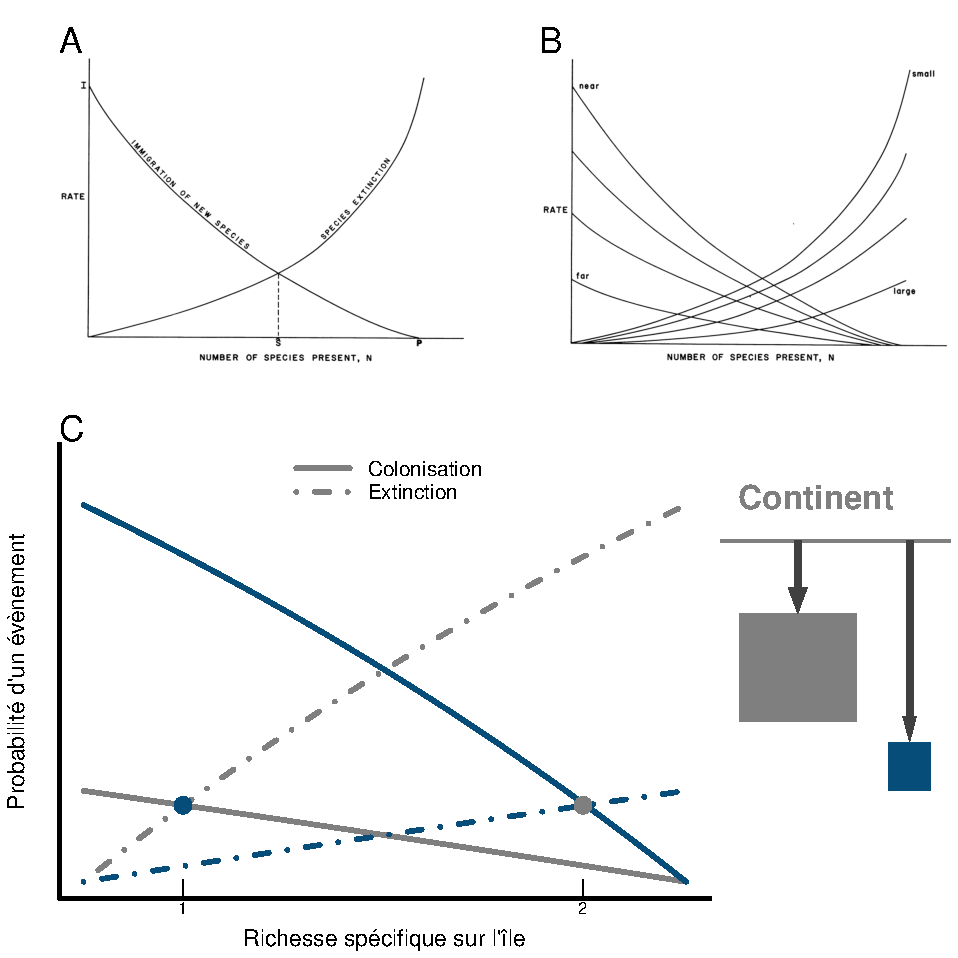
\includegraphics{fig/fig1.pdf}
\caption{\textbf{La Théorie de la biogéographie des Iles.} L'évolution
des taux de colonisation et d'extinction est présentée pour deux îles
aux caractéristiques différentes. Les tailles relatives des îles et les
distances qui les séparent du continent sont schématisées à droite du
graphique, les couleurs associent les îles à leurs courbes respectives.
Le pool d'espèce régional (\(P\)) est constitué de 100 espèces, les taux
de colonisation et d'extinction sont exprimés en terme de probabilité
d'évènement. Les points où colonisation et extinction s'équilibrent sont
marqué par les symboles en gris.\label{fig:figMW}}
\end{figure}

\subsection{Environnement abiotique et distribution des espèces}

Les atouts actuels de la biogéographie sont 1- une quantité importante
d'information relative aux présences d'espèces et au climat et 2- des
modèles corrélatifs puissants qui décrivent précisément le lien entre
l'espèce et son environnement abiotique. Le terme abiotique peut prêter
à confusion dans la mesure où les espèces elles-mêmes peuvent modifier
des variables dîtes abiotiques. Par exemple, les végétaux peuvent avoir
un grand impact sur les variables abiotiques locales comme la
température et l'humidité du sol \cite{Breshears1998}. Certains auteurs
font une distinction précise en utilisant les termes de
\textit{scenopoetiques} pour les variables environnementales sur
lesquels les espèces ne peuvent influer et de
\textit{dynamiquement liées} pour les autres \cite{Peterson2011}. Nous
occulterons volontairement ces-dernières, l'environnement abiotique dont
il est ici question n'est donc pas dynamiquement lié aux espèces.

Le premier pas pour expliquer la répartition des espèces est alors la
recherche des variables environnementales les plus discriminantes pour
comprendre la présence des espèces en un lieu donné \cite{Kearney2004}.
Au coeur de cette démarche existe un enracinement biologique profond. En
effet, pour pouvoir s'installer sur un territoire donné, une espèce
présente un certain nombre d'exigences physiologiques. De manière
générale, l'espèce doit pouvoir répondre à l'ensemble de ses dépenses
énergétiques pour survivre et éventuellement se reproduire
\cite{Holt2009a}. La dernière condition n'est pas indispensable : la
présence d'une espèce peut résulter d'une permanente colonisation
\cite{Leibold2004}. Cet espace des variables environnementales dans
lequel une survie d'une population est possible, nous l'appellerons
niche écologique. Ce terme est l'objet de vif débat \cite{Chase2003} que
nous éviterons en rappelant la définition employé. Nous palerons ici de
niche fondamentale pour désigner l'ensemble des variables
\textit{scenopoetiques} et niche réalisée lorsque la composante biotique
intervient, même indirectement.

De nombreux travaux démontrent que les variables environnementales ont
un grand pouvoir pour expliquer la présence des espèces
\cite{Engelbrecht2007}. A partir de cette connaissance, il suffit de
projeter l'espace environnemental sur l'espace géographique. Pour
prédire la répartition de la biodiversité de demain, on couple des
modèles d'évolution de l'environnent abiotique avec cette projection.
Cette démarche rencontre actuellement un grand succès, les changements
globaux induisant un effort de recherche important dans le domaine
\cite{Thomas2004,Thuiller2011}. Il est crucial que les modèles
théoriques tel que le modèle de la TIB s'approprient le concept de niche
fondamentale sous une forme simple mais cohérente. C'est en tout premier
lieu par l'utilisation des variables environnementales abiotiques que
les modèles théoriques en biogéographie peuvent démontrer leur
pertinence et attester de leur proximité avec les modèles plus
corrélatifs et plus appliqués.

L'emploi des variables abiotiques seules pour comprendre la répartition
des espèces demeurent problématique. Alors qu'il semble raisonnable de
considérer des facteurs tels que la présence d'eau, de lumière et la
température pour expliquer la distribution des végétaux, lorsqu'il
s'agit d'espèces de niveaux trophiques plus élevés, les seules données
de l'environnement abiotique ne suffisent pas
\cite{Gravel2011b,Godsoe2012}. Nous considérons, pour alimenter la
réflexion, un exemple simple : un prédateur spécialiste et sa proie. De
par l'étroite relation que les deux espèces entretiennent, il est peu
efficace de regarder les seuls facteurs abiotiques pour comprendre la
répartition future du prédateur. Il est alors plus pertinent d'examiner
la répartition future de la proie et de s'interroger sur les
possibilités de dispersion du prédateur.

\subsection{Réseaux d'interactions : interdépendance des espèces}

Il est difficile de concevoir les espèces comme indépendantes, elles
partagent des espaces communs et des sources d'énergie, elles échangent
de la matière, elles sont en permanentes interactions. Ces relations
intra et inter spécifiques sont au coeur de l'écologie. En dynamique des
populations, sont arrivés très vite des modèles classiques attestant les
relations proies-prédateurs témoignant de l'importance de traiter la
démographie de différentes espèces simultanément . L'écologie des
réseaux pose des questions fondamentales comme celle de la stabilité des
écosystèmes au regard de la structure des réseaux \cite{Allesina2012}.
Au delà des relations trophiques, les interactions peuvent se manifester
sous de nombreuses formes \cite{Kefi2012}. Le mutualisme, le
commensalisme et la compétition sont des relations qui affectent la
démographie des espèces sans que l'une d'entre elles se nourrisse d'une
autre. La représentation en réseau des interactions est un outil
puissant pour synthétiser la complexité des écosystèmes
\cite{Sole2006,Pascual2006}. Ils sont représentés par la matrice de
communauté qui résume l'effet démographique des espèces par pair. Cette
matrice renferme des informations précieuses telles que la connectance
(mesure du nombre de liens constatés rapporté au nombre de liens
possibles), la topologie des interactions entre espèces \cite{Sole2006}
et les effets indirects \cite{Bender1984, Montoya2009}.

Les interactions intra et inter spécifiques constituent un facteur
rapidement pressenti comme responsable de la distribution spatiale des
espèces \cite{Levin1974}. L'interdépendance des espèces conditionne, en
effet, l'aspect favorable de l'environnement au sens large (biotique et
abiotique). Ainsi Godsoe \textit{et al.} 2012, mettent en équations le
caractère favorable de l'environnement pour une espèce donnée en terme
de probabilité de présence d'une autre espèce et de la nature de leur
interaction \cite{Godsoe2012}. De même, Holt et Barfield 2009 montrent
l'impact de la prédation sur la répartition d'espèces en compétition
\cite{Holt2009} insistant ainsi sur le rôle majeur des interactions.
Davis \textit{et al.} 1998 ont montrés que, pour trois drosophiles en
compétition, l'effet d'un parasitoïde n'est pas le même le long d'un
gradient selon que les espèces sont seules ou ensemble \cite{Davis1998}.
Récemment, des efforts ont été réalisés pour mettre en évidence
l'importance de l'interdépendance des espèces dans les données aux
larges échelles spatiales \cite{Gotelli2010}. On trouve actuellement
dans la littérature une grande motivation pour les intégrer dans les
modèles de distribution d'espèces \cite{Kissling2011, Guisan2011}. Des
efforts théoriques sont encore nécessaires pour arriver à de telles
approches. Néanmoins, rapprocher différents champs de l'écologie peut
s'avérer d'une utilité majeure. Jabot et Bascompte \cite{Jabot2012}
2012, ont d'ailleurs montré l'importance des interactions pour
comprendre la distribution des espèces en rapprochant écologie des
réseaux et un modèle de metacommunauté. De même Gravel \textit{et al.}
2011 \cite{Gravel2011b} introduise l'interdépendance proie-prédateur
dans le modèle classique de MacArthur et Wilson menant aux prémices
d'une théorie trophique de la biogéographie des îles.

L'ajout des interactions dans un modèle incluant l'environnement
abiotique interroge la relation que les deux processus entretiennent. Si
les espèces n'ont pas les mêmes performances dans différents milieux du
fait de leur physiologie, pour les mêmes espèces considérées, les
réseaux n'ont pas de raison d'être identiques d'un milieu à un autre.
C'est sur ce fait que Poisot \textit{et al.} 2012 ont proposé une mesure
de dissimilarité des réseaux \cite{Poisot2012}. Defossez \textit{et al.}
montrent que les interactions négatives entre l'hêtre commun
(\textit{Fagus Sylvaitca}) et les micro-organismes du sol diminuent avec
l'altitude \cite{Defossez2011}. Ainsi, les contraintes biotiques sont à
relier à l'environnement \cite{Brooker2006,Canham2006} et un modèle
intégratif doit donner un cadre cohérent à ces rétroactions entre
processus. Enfin, l'importance des interactions est à mettre en relation
avec l'échelle considérée \cite{Peterson2011}. Pour deux espèces en
interaction, plus l'échelle d'étude est large, moins les effets des
interactions locales sont susceptibles d'être capturés, le pouvoir
explicatif de la présence d'une espèce sur l'autre peut être alors
discutable \cite{Araujo2007}. Comprendre quels sont les processus à
prendre en compte aux différentes échelles spatio-temporelles et
comprendre comment le changement d'échelle affecte nous prédictions est
aussi un véritable challenge en biogéographie \cite{Martinez2012}.

\subsection{Plasticité phénotypique et processus évolutifs}

La vie telle que nous la connaissons pérennise l'information accumulée
au cours du temps via à un support moléculaire, l'ADN. Cette molécule
peut 1- renfermer une plasticité phénotypique offrant aux espèces des
possibilités pour faire face aux stress environnementaux et 2- subir des
altérations, des mutations, dont le relative avantage apporté peut
assurer une survie accrue. Les espèces sont donc elles-mêmes porteuses
potentielles de réponses face aux changement actuels
\cite{Parmesan2006,Lavergne2010}. La plasticité phénotypique permet une
réaction rapide des espèces à des changements environnementaux soudains.
Tingley \textit{et al.} 2009 ont ainsi montré que sur 53 espèces
d'oiseaux étudiés dans la Sierra Nevada, 48 ont colonisé de nouveaux
sites où les conditions de température et de précipitations leur étaient
plus favorables \cite{Tingley2009}. Les mutations sont quant à elles des
évènements relativement rares qui interviennent potentiellement à chaque
génération, leur fréquence est donc dépendante, en premier lieu du temps
de génération mais aussi de la tolérance des systèmes de réplication du
matériel génétique. Pour des espèces aux temps de génération court, les
processus micro-évolutifs peuvent donc être déterminants. Ainsi, Balanyá
\textit{et al.} 2009 ont montré des changements notables dans le
génotype de \textit{Drosophila subobscura} en 24 années avec des
génotypes de basses latitudes plus répandus en réponses au changements
climatiques.

Il est capital de ne pas oublier les processus évolutifs dans un modèle
de biogéographie afin d'envisager correctement la biodiversité de demain
\cite{Sexton2009,Lavergne2010}. La nature des processus à prendre en
compte est dépendante de l'échelle de temps considérée. Ainsi, si l'on
souhaite retracer l'histoire évolutive d'une région, les aspects
adaptatifs relevant de la micro-évolution sont moins pertinents que les
processus évolutifs de longue portée modifiant profondément les espèces.
Il faut, à ce propos, rappeler que l'évolution peut conduire à un
enrichissement du pool d'espèce d'une région donnée
\cite{Rosindell2011,MacArthur1967}. Les mutations accumulées dans une
population isolée géographiquement peuvent conduire à une
incompatibilité reproductive avec les populations du pool dont elle est
issue. Il y a alors spéciation, la biodiversité est augmentée. A court
terme, les processus longs de spéciation peuvent être occultés mais
prendre en compte les phénomènes d'adaptation et les processus
d'évolution des espèces au temps de générations court est important. Il
est aussi important de distinguer les réponses phénotypiques des
réponses évolutives, les premières pouvant être plus rapide mais à
porter moindre que les secondes plus lentes \cite{Gienapp2008}.

Les processus évolutifs peuvent être favorisés par les changements
environnementaux mais également par les interactions entre espèces
\cite{Tingley2009}. Les étroites relations entre espèces peuvent
favoriser ou contraindre les réponses évolutifs, qui elles-mêmes peuvent
altérées ces interactions, il existe de fait des rétroactions
permanentes entre évolution et écologie \cite{Post2009}. Yoshida
\textit{et al.} 2003 montrent que la réponse des algues vertes
unicellulaires \textit{Chlorella vulgaris} aux rotifères
\textit{Brachionus calyciflorus} conduit à un changement dans la
fréquence et la phase des cycles de la dynamiques proie prédateur
\cite{Yoshida2003}. L'ensemble des trois éléments jusqu'ici évoqués
(environnement abiotique, interaction, évolution) peuvent également être
étroitement associé. Grant et Grant 2006 rapportent le cas de la
compétition entre trois espèces de pinsons (dits de Darwin) sur l'ile de
Daphne (Galapagos) qui engendre une modification de la taille de leurs
becs. Cette évolution liée à la compétition est elle même reliée à
l'environnement abiotique car, par l'abondance ou l'absence de
précipitations, il détermine la disponibilité des ressources et donc
l'intensité de la compétition \cite{Grant2006}. A travers cet exemple,
nous comprenons l'importance d'inclure l'ensemble des différents
processus pour construire un modèle intégratif en biogéographie. Un tel
modèle serait capable, par exemple, de renseigner les risques
d'exclusion compétitive dans l'exemple décrit par Grant et Grant.

\subsection{Traits fonctionnels}

Les traits fonctionnels sont des propriétés mesurables sur les
organismes en relation avec leurs performances et leur rôle dans
l'écosystème \cite{McGill2006}. Les traits étudiés peuvent être de
différentes natures, 1-morphologiques : taille de différentes parties du
corps, position des yeux, taille des oeufs chez les organismes ovipares,
taille des graines pour les végétaux, 2- physiologiques : taux
métaboliques de bases, stœchiométrie (rapport de la concentration entre
divers éléments qui compose l'organismes)
\cite{McGill2006,Albouy2011,Litchman2008}. Un ensemble approprié de ces
propriétés peut être un outil puissant pour décrire un ensemble d'espèce
dans un même espace. Leur proximité dans l'espace des traits est alors
un indice précieux d'une proximité fonctionnelle. Ainsi, à l'aide de 13
traits ecomorphlogiques, Albouy \textit{et al.} 2011 parviennent à
prédire les guildes trophiques de 35 espèces de poissons de la
Méditerranée \cite{Albouy2011}. Edwards \textit{et al.} 2013 montrent
que l'effet saisonnier sur une communauté de phytoplancton dans la
Manche peut être capturé à l'aide de traits décrivant : le taux maximal
de croissance, la compétitivité pour la lumière et l'azote
\cite{Edwards2013}. La distribution des traits fonctionnels au sein de
la biodiversité est aussi une entrée de choix pour réfléchir quand à la
fragilité potentielle des fonctions remplies par les écosystèmes
\cite{Mouillot2013}. \%DG: je comprends cette citation de Mouillot, mais
juste une mise en garde contre ce type de référence. Mouillot se base
sur l'hypothèse que les traits nous informent du fonctionnement, sans
jamais documenter cette relation. Ce qui est souvent le cas, et par
conséquent contribue à bâtir des mythes dans la littérature qui à
l'occasion ne sont pas toujours bien appuyés. L'approche par traits est
un bel exemple, on a édifié rapidement une structure conceptuelle sur
les traits, mais on n'a pas solidement appuyé le concept sur de bonnes
bases empiriques.

L'approche de la biodiversité par les traits fonctionnels est plus
quantitative que l'approche taxonomique et permet de déduire un grand
nombre de propriétés en se passant de la connaissance de leur identité.
Ainsi McGill, dans son article d'opinion de 2006, propose une approche
nouvelle de l'écologie des communautés qui transforme les questions
centrées autour des espèces par des questions qui interrogent la
répartition et la variabilité des traits \cite{McGill2006}. L'emploi des
traits fonctionnels est en fait un appel à une écologie plus mécaniste,
qui se penche sur la physiologie des organismes, en prend les faits les
plus importants (relativement au problème traité) pour les placer dans
un espace de traits commun. Cette approche est aussi en lien avec la
controversée théorie métabolique en écologie
\cite{Brown2004, Price2012}. Dans cette théorie un certain nombre de
grandeurs (comme le taux métabolique) sont reliées à la biomasse
corporelles de l'adulte, fournissant ainsi en un seul trait de
nombreuses relations pour des groupes d'organismes très différents. Par
ces nouvelles approches, l'espérance de s'extraire de la seule identité
des espèces est accrue, l'idée d'avoir des règles générales se
concrétise.

Dans une théorie intégrative de la biogéographie, les traits
fonctionnels peuvent être un pivot très intéressant pour rassembler les
différents concepts que nous avons développés dans les paragraphes
précédents. Les traits peuvent tout d'abord être mis en relation avec le
milieu abiotique. Le taux métabolique ou encore la sensibilité à la
sécheresse sont des indices performant pour décrire la survie dans un
milieu donné \cite{Kearney2004,Engelbrecht2007} que l'on peut capturer
sous forme de traits. Kearney \textit{et al.} 2010 propose une approche
prometteuse dans laquelle, l'environnement physique, la disponibilité
des ressources et la dynamique énergétique sont reliées par les traits
fonctionnelles le tout aboutissant à un modèle de distribution très
mécanistes. La structure d'un réseaux peut également être dérivée à
partir de l'espace des traits. Dans leur méthode proposée cette année,
Gravel \textit{et al.} infèrent les paramètres du modèle de niche de
Williams et Martinez \cite{Williams2000} à partir des relations de masse
du corps entre proie et prédateurs \cite{Gravel2013}. Ils sont alors en
mesure de dériver un réseau global pour un ensemble d'espèce donné.
Enfin, en tant qu'expression phénotypique, les traits fonctionnels sont
soumis aux processus évolutifs. Sur les temps longs, l'expression de
l'évolution résulte en la modification progressive des traits qui se
répercute sur l'ensemble des propriétés qui en découle. Ainsi la
considération d'une modification des traits est une approche simple et
réaliste pour introduire les processus évolutifs et leurs conséquences
\cite{Guill2008,Loeuille2005}.

\subsection{Inférence en biogéographie}

Rappelons les objectifs de la biogéographie : décrire et comprendre le
lien entre le vivant et l'espace sur la Terre. Le coeur de l'inférence
en biogéographie est donc de trouver les variables les plus pertinentes
pour la répartition des espèces. Pour cela, les données spatialisées de
présence ou d'abondance des organismes étudiés sont mises en relation
avec des variables prédictives également spatialisées
\cite{Guisan2005,Peterson2011,Elith2009a}. Idéalement, les échelles
spatiales coïncident, sinon des transformations des données sont
nécessaires. Si la variabilité capturée est satisfaisante, la
combinaison retenue de variables explicatives éclairent alors les motifs
de la présence des espèces en un lieu donné. Nous retiendrons le nom de
modèle de distribution des espèces (MDE) pour référer à cette démarche
de modélisation générale. Il y a cependant de nombreux aspects à
discuter relatifs aux variables explicatives employées. Les MDE ont
fourni des exemples attestant de leur pouvoir à décrire la niche
fondamentale pour expliquer les présences des espèces
\cite{Kearney2004}. Si l'on considère des espèces mobiles, il est
problématique de négliger leur mouvement, la dispersion et ses limites
doivent alors être incorporés dans les modèles de distribution
\cite{Gotelli2009}. De même, les espèces interagissant entre elles,
elles influencent leurs distributions. Utiliser une espèce en tant que
variable explicative pour la présence d'une autre peut s'avérer
pertinent \cite{Araujo2007,Pearson2003} mais soulève la question
suivante: que faire lorsque nous essayons de prédire simultanément la
présence de deux espèces dont les observations résultent elles-même de
leurs échanges ?

Dans le contexte actuel des changements globaux, il y a une
concentration des efforts pour mieux cerner l'ensemble des réponses
possibles des espèces face aux changements globaux \cite{Bellard2012}.
En guise de réponse, les MDE deviennent plus intégrateurs et de
nouvelles approches émergent \cite{Kissling2011}. Ainsi, Guisan et
Rahbek 2011 proposent une démarche alliant les prédictions faîtes par
les MDE sur un ensemble d'espèces et celles données par une approche de
modélisation macroécologiques s'appuyant sur des règles de coexistence
dans une unité géographique donnée \cite{Guisan2011}. Le travail de
Gotelli \textit{et al.} est également un exemple de démarche intégrative
où un nombre important de processus peuvent être inclus via un système
de combinaison de scénarios et tester par simulations stochastiques
\cite{Gotelli2009}. Enfin, en construisant des réseaux basés sur la
cooccurrence des espèces, Araújo \textit{et al.} revisitent le problème
de l'interdépendance des espèces \cite{Araujo2011} : ils s'interrogent
sur la résistance des réseaux de cooccurrence obtenus face aux futurs
changement climatiques, ils mettent ainsi en évidence des risques accrus
de perte des espèces les moins connectés (celles qui cooccurent moins).
Ces travaux témoignent de la volonté d'une biogéographie intégrative.

Malgré leurs performances, les modèles de distribution actuels utilisés
pour construire les scénarios de biodiversité de demain souffrent
vraisemblablement d'un manque de théorie sous-jacent
\cite{Beck2012,Lomolino2000}. La nécessité d'une approche théorique pour
aller vers des approches plus appliquées est fondamentale, en
témoignent, par exemple, l'histoire de la théorie de la biogéographie
\cite{MacArthur1967} et de la théorie métabolique \cite{Brown2004}. Dans
notre cas, partir d'une construction progressive assemblant les
différents processus décrits ci-dessus nourrit, dans un premier temps,
la réflexion sur l'ensemble des retroactions que peuvent exercer les
différents processus les uns sur les autres\cite{Thuiller2013}. Dans un
second temps, le questionnement sur les échelles des phénomènes peut
amener à isoler les processus que les futurs MDE ne doivent pas occulter
au regard des échelles spatio-temporelles qu'ils considèrent.
Troisièmement, les modèles théoriques fournissent des hypothèses à
confronter aux faits, ce qui permet de conforter ou d'infirmer la
théorie. Enfin, si l'agencement des processus entre eux est bien
expliqué, de la théorie peut émerger de nouvelles méthodes pour traiter
les données.

\subsection{figures envisagées}\label{figures-envisaguxe9es}

\begin{itemize}
\tightlist
\item
  les problèmes d'échelles (figure qui cmontrent des paramètres qui
  captures si ou ça\ldots{})
\item
  les reltions ``solides'' de la biogéographie
\end{itemize}

\subsection{L'espace en liu
2même\ldots{}}\label{lespace-en-liu-2muxeame}

\subsection{Remarques}\label{remarques}

``It just so happens that some people find it easier to think about
things in terms of x's and y's, and other in terms rabbits of and
lynx.'' MCann Preface

L'objet de ma thèse est sur la sidtibution des espèces et les
interactions et ce que la comjonction de tout ça. Elle est le plus
souvent des articles qui sont de mon point de cue plus une reflexion des
iudées et pas nécesairemnt des démonstrations formelles et fermées mais
la tentative de trouer des ouvertires d'appliquer des outils de msnière
un petit peu différete pour donner, ce que cherche ltous doc àdonner de
l'originalté é mon traviell. Chemin faisant j'ai passé bien du tenmsp
derrière l'ordi pour lere anayser faore des modèles mathématiques
ensuite implémenté in silico. Dans cette introduciotn je ne peux donc
pas faore l'impasse sur une mise en contexte générale de la
biogéogrpahie avec ces apports historiques ces contraintes mais aussi
l'age dans lequel nous sommes et les défis mais aussi toutes les aspects
d'ordres computationnelle parler de modélisations de ces enjeux et
valoriser les modèles thérqies fondamentaux qui s'éloignent parfois de
la éalité mais sans jamsi la déconsidérer.

Les paragraphes sont pour l'instant mis à titre indicatif avec aucune
contrainte en terme de taille c'est juste pour y mettre les idées qui me
viennent.

Dans la premièr partie de cette introduciton je fais un tour très large
de notion d'horizon biogéogrpahie / pilier théoriqe / besoind
d'hypothèse en biogéograohie et finir sur la modélisation. Pour dans un
deuxième temps les articuler autour de questions précises

\subsection{La distribution des espèces des faits et des
causes}\label{la-distribution-des-espuxe8ces-des-faits-et-des-causes}

Le concept récent de biodiversité.

However ecological equivalence in

``the niche is a mapping of population dynamics onto this space''
({\textbf{???}})

\subsubsection{De l'émerveillement}\label{de-luxe9merveillement}

=\textgreater{} Partir de Wallace. L'inventaire de Wallace est
impressionnant cet

\subsubsection{Des causes / des
mécanismes}\label{des-causes-des-muxe9canismes}

vers le fonctionnemt des ecosystèmes levier d'action vers une approche
plus utilitariste mais qui donne uns certaine proximité avec les
eécosytèmes Loreau et al. (2001)

\subsubsection{Challeng vers un espoir de
généralisation}\label{challeng-vers-un-espoir-de-guxe9nuxe9ralisation}

\subsection{Une question d'échelle}\label{une-question-duxe9chelle-1}

Se problème est d'une grande importance. L'écologie porte sur l'ensemble
du monde vivant quelquees soiten leur taille mais les différent champs
ne sont pas toutes relatoves à la m\^{}me échelle alors il y a bien els
échelles de temps, les echelles spatiales mais il y a le lével
d'organisation. Il est bien inportant de comprendre celad !

Un scéhma avec des variables qui émergenet ave différemts paramères et
quelques éxemelpme de théorie! (DEB Evolution foodweb\ldots{}) et
l'action de

Repartition des especes des passges histroqiere dans l'origin des
espèces et dans Wallace. Le principe même de l'écologie (la definition
de ecologie).On arrive à l'idée de ;la niche. Exemple histriques. Dans
son ouvrage, le grand biogéographe Wallace reconait en introduction le
caractère facinant de la réaortition de la biodiversité des îles avec
des faot intriguant wuant à la faune et la flore. Ainsi il constate
qu'il peut y avir plus deux différence entre île très éloigné et deux
île s très proche. Il écrit que la faune et la flore sont plus
dissimilaire entre ldeles deux piles des Galapagos Bali et Lombik
qu'entre Hokaido (Yesso) et La grand bretagne ouy encore la Nouvelle
Zéland et l'Australie,

Exemple classique de grinnel et des Trasher + evolution avec les
charcter displacement.

Nous accumulons des évidences quand aux impact du changement
anthropique. A diiférentes échelles la diminution de la biodiversité,
chngemnt en compoisiton Taranu et al. (2015) De Roos et al. (2008)

\subsection{P2}\label{p2}

La niche c'est quoi on en a deux definition ultr classique mais elles
sont très porblématiques. Il y a des tentatives de synthèse mais le
problèmes est toujours là.

Partir du development de la niche et des hypotheses clef comme
l'heterogeneité spatiale qui peut accroitre la biodiversité un exemple
c'est les ecoulemnents à petites faible echelles de l'hydrologie niche
hdrologique à fable échelles Letten et al. (2015) repartition
hydrologique les hypothèses sont que qui explique celon les différentes
besoin des espèces (principes de la niche) que besoin différemtes me
répartition des espèces. Cette idées est

A large espes répartition de la biodiversité on quantifie la différence
depuis les mesures classiques Simpson, alpha gamma beta qui sont
étendues au réseau Poisot et al. (2012). Mais quand on chnage d'echelle
on arrive rarement à quelques choses de concluant pour l'integration des
interactions. Pourtant il ya des exemples convaicant comme celui de
Gitelli.

Les interactions c'est quoi ce qu'on en fait.

Les interactions quelles pourrait être leur conséquence à large échelle
?

Mais au-dela de cela il yt a un besoin de règles. L,écoligies cherche
ces règles et essayes de faire le max sans trip de succès. Les traits
sont un gran despoir. On a besoinde rule on reste descriptive il y a des
relation EH-Bioversité, SAR, Diversité-équilibre diversité
fonctionnenemnt qui sont partielelemnt reliées et des théries débat
theories neutre theéor de la niche Stein et al. (2014). Dans cette
review Stein et al. (2014) montre que vegettaion est inportnates ce qui
eimplique des inbteractions. Théorie allométrique prometteuse en ce sens
qu'elle loi physiques. Différents concept autrour d'une même notion sur
plusieurs paradigme pour une même notion sur les metacommunity Leibold
et al. (2004) il peuvent co-exister mais faudrait les savoir ce qui fait
qu'on a pus l'un ou l'autr.

Exemple histroqies les Pinsons de darwin (cdf mon devis.) Les processus
évolutifs peuvent être favorisés par les changements environnementaux
mais également par les interactions entre espèces \cite{Tingley2009}.
Les étroites relations entre espèces peuvent favoriser ou contraindre
les réponses évolutifs, qui elles-mêmes peuvent altérées ces
interactions, il existe de fait des rétroactions permanentes entre
évolution et écologie \cite{Post2009}. Yoshida \textit{et al.} 2003
montrent que la réponse des algues vertes unicellulaires
\textit{Chlorella vulgaris} aux rotifères
\textit{Brachionus calyciflorus} conduit à un changement dans la
fréquence et la phase des cycles de la dynamiques proie prédateur
\cite{Yoshida2003}. L'ensemble des trois éléments jusqu'ici évoqués
(environnement abiotique, interaction, évolution) peuvent également être
étroitement associé. Grant et Grant 2006 rapportent le cas de la
compétition entre trois espèces de pinsons (dits de Darwin) sur l'ile de
Daphne (Galapagos) qui engendre une modification de la taille de leurs
becs. Cette évolution liée à la compétition est elle même reliée à
l'environnement abiotique car, par l'abondance ou l'absence de
précipitations, il détermine la disponibilité des ressources et donc
l'intensité de la compétition \cite{Grant2006}. A travers cet exemple,
nous comprenons l'importance d'inclure l'ensemble des différents
processus pour construire un modèle intégratif en biogéographie. Un tel
modèle serait capable, par exemple, de renseigner les risques
d'exclusion compétitive dans l'exemple décrit par Grant et Grant.

La puissance de la Biogéographie est aussi sont implications dans des
cas très concrets Cirtwill and Stouffer (2015) mais aussi ne puissance
exploratoire théoriques Gravel et al. (2011) Cazelles et al. (2015) des
îles

l'idée des interactions à déjà montré ça pertinence sur plusieurs
exemples. Cirtwill and Stouffer (2015)

\subsection{Les relations de la
biogéographie}\label{les-relations-de-la-bioguxe9ographie}

Relation diversiyté des habitats Relation aire quantitié d'espéces SAR /
relation de la biogeograhies des îles Compromis entre aire et
hétérogénéité\ldots{}

\section{Conclusion}\label{conclusion}

Generalist consumers should typically be weakly coupled to any one of
their prey populations because, when feeding on many different species,
they cannot be strongly coupled to any one of them Murdoch et al. (2002)

\section{Predire la répartiton futrure des
espèces}\label{predire-la-ruxe9partiton-futrure-des-espuxe8ces}

On fait des atlas des 2 des entités avec un einertoie historqiue mas
est-ce là important pour comprendre le réseuax ? Hortal et al. (2011)

Bien sur un objectif central est d'être en mesure de prédire la
répartitopon des espèces L'ecéologie avance avec des rêves mais des
pièce manquante le lien entre les espèces et le foodweb le lien entre la
présence des espèces et le fonctionenent. Il y a des problèmes
fincdamnentale et qui sont complexes. Par exemple les espèce peuvent
avoir été invasives et causé des dégâts sur les ecosystèmes, il y a les
exemples de l'aAustraile véritable laboratoire avec les boeufs les
crotets els inporatation mais d'un autre côté ça fnctionne encore.

Pour la prédicitons des distribution d'espèces la processus et simple et
bien expliqué dans le libvre de Peterson. Finalemt l'eercie consiste à
trouver les contraintes evironemntale qui sont les bonnes et ce placé
ensuite un certai nombre de contrainte peuvent être les même il y a de
nombreux avantages à une telle métyhdoes compréhensiblem empiriqument
fond.é, intuitibenbt quand on va dans des endroits humides ou sec o
connait bien la différence de type d'cosytèmes mais il faut rajouter
bien des couches. Ainsi la possibilité de colonisaton 'est pour ça que
des ecosystèmes sont aussi éloignés mais pas les mêmes espèces
dessous.Rajouter l'histoire evolutive pour bien comprendre la
co-evolution des humming bord 9cf mail de Bo)

La bonne unité d'analyse ? D'où parti r?

=\textgreater{} Faire un exemple tout automatiser et stocker sous
Github.

Les système écologique sont des systèmes trasitoire par excellence et on
veux qu'il soit satbel mais il y a une contingence encore assez dure à
admettre les système que nosu observons sont on cherche à les modéliser
mais il faut pas oublier qu'ils ne resterin t pas et qu'ils sont
peut-être entrain de disporaître que les moteurs de l'évolution rebat
lenteemnt les cartes

\subsection{Modéliser}\label{moduxe9liser}

`The types of questions we pose and the types of observations we make
bear witness to our preconceptions. There is no way to get rid of them.
There is nothing wrong with this, but we should be aware of it. When we
look around us we actually see mirrors of our ideas. We can try to
change ourselves on the basis of what we see, but we cannot do without
the projections we impose on reality. Observations and statements span
the full range from facts via interpretation to abstract ideas. The more
abstract the idea, the more important the mirror effect.' Kojjman

Tentatove de modéliser toutes les espèces à l'échelles de la terre
entière alors qu'on est capable de généres dynamiques chaotiques à
partir d'une seule espèces. Attention je ne veux pas dire que les
premières tentatives sont vaines et je ne méprends pas sur la dynamqiue
chaotique, j'indique simplement que s'il y a des cas de population
isolés où a dynaqieu ne peut être connu à sans une précision initiale
sur les coniditon initiales on peut se demander comment cela peut être
extrapoller. Mais la enocre il y qeulques chsoses d'intéressant
cconneitre abondance compotioon excate peucvent être connu à une èchelle
de temps courte = métérolge alors peut-être qu'au échelle plus large des
entité plus grande = climatologie de la biodiversité !

approhe modulaire =\textgreater{} rupture de symétrie

J'explore quelques dualié propre à l'acte de modélisation que j'applique
ultiment au champd e la biogéogroahie

\subsection{Correlative / Mechanism}\label{correlative-mechanism}

\subsubsection{Règle et containgence}\label{ruxe8gle-et-containgence}

Finalemnt se problème est aussi lié au problème d'échelle de travail !
il y a un problème d'échelle

Quand on se tourne vers les sciences de l'écomomie il y a un bon jeus de
mots que j'ai entendu sous deux formes : - Les physiciens oont 5 règles
pour expliquer 95\% univers et les 95 rèle pour 5\% - Les économistes
ont pédit 12 des trois dernière crises éconimoqe

Il y a un sentiment partagé avec l'écologie (beaucouoe en commun dans la
raci) administration/gestion de la maison que l'on recent plus dans le
trerme familier que / c'est la science de la maison, de l'habitat. et
une compléxité une légère jalousie des physiciens se serait qui ont des
théories qui ont prédi des objets à une époque où pas les moyens de
faire les intslallation Boson Onde rgavitationelle ou encore expliquer
la loi de fourier à partir de la mécanique statitsiqes

Rassurons nous les physiciens ont encore bien des parties sonmbres
àexplorer : matière noire et energie noire et du boulot en masse pour
ecologues / economistes peut-être que les foralimes que nous empreintons
à ces disciplines ne sont pas les bons\ldots{} Comme dit le phylodophe
Sachs dans sa biodiversité c'est trop historiques qu'un concepte comme
le fitness n,est peutêtre pas bien mis en equation dans une forme
physique

\subsubsection{Un acte d'abstarction pour des défis très
concret}\label{un-acte-dabstarction-pour-des-duxe9fis-truxe8s-concret}

ce n'est pas objectif, c'est se placer dans un cadre et c'est une façon
de contruire le raisonemet. Exemple on peut vouloir modéliser la
robabiliter d'interaction et alors uon peut commenceer par une
probabilité de rencontre qui est simplemnt la probabiliter de se
detecter mais qui pourrait être calcluer de manière complexe ou alors
juste un paramètre.

Il y a différent niveau la modelisation a pour but de donner une idée
mais n'oublions as qu'il existe une progression, un raffinement et
qu'ultimement, le réalisme de la simulation permet d'obetnir
préscisement le phénomène données et on peut aller très loin à partor
d'imagination d'un aller retour entre le réel et l'espace dans lequel on
se place pour modéliser.

Même sur des dynamiqeues d'espèce l'échelle

Prendre quelques

Devons-nous prendre un modèle taille ou agr structuré quand on cherche
la distibution des espàces à large échelle

Des courbes à fitetr qui sont parfois les m\^{}mes et donc peut
infornatives\ldots{}

prendre deux oiseaux il y a une relation phylo mais ecologiquenent qui
est le plus proche ? Qui a quelle rôe ? Les traist permettent cette
abastraction qui ne doit pas non pplus laisser de cote la phylo, il faut
bien sur regarder tout pour avoir l'image complete

Un modèle existe en lui soi on pourrait se demander Evaluation au regard
de sa perfomnce

\subsubsection{Deterministes ou
stochastiques}\label{deterministes-ou-stochastiques}

Il n'y pas de maeilleur manière les stats c'est sur du stochastique et
on peut mettre du stochatci avec une variance c'est le r.sultats d'un
théorème maus il en est aps moins que variance es quelqeues choses d
etrès util et au bour aller des moi On peut avoir un modèle détermicites
qui explique tout mais

Le hasard est qquelques choses qui est dans le dé ce que Monod dans le
hasard et la cnécessité appelle un ahasar opétaionnel certain pense
alors que le dé est un faux hazard que la détermination des lois de
Newton et des forces inital est totallemnt déterminée et on peut donc
prédire que le résulat du dé. Cependant c'est l'ensemble croisé de série
de contingence qui amènent au hasrad et dans une partie de Yatz il sera
bien difficile d'obtenir un score souhaité\ldots{} Mais le hasard pur
existe-t-il ? Dans l'oeuvre de Momod le hasard existe et c'est l'ADn
polymérase à l,origine des mutations qui en est l'expression. mais
l'ensemble des série de combinason

Lien entre les deux Une manière de voir les choses est de donenr par
Clark (et repris par Dom) pou on essaye

Clark a suggérez que stochastique n,est pas savoir et que le but c'est
de passé du pas au maximum vers le détermiste. Dans elur défendse de la
la théroy neutre Rosindell et al rétoquent que c'est plus subile il y a
des modèles dtermisites chatosque (et dont les développemtn avancé font
au propriété statistique des attracteurs) quer cela de même Gravel et
collègues.. rreprche que. Modèles en plus validée par des stats qui
reposent sur des stochsiques. Argument d'Einstien Dieu ne jue pas au dé
face à la quantique qui au final alors mêe que le la gravitaté générale
sans hazard pure sera fause. Le chat de Shrodinger est peut-être vivant
ici mais il est mort dans un autre univers.

Produire variance et moments d'ordre supérierus\ldots{}

Dans mon premier chapitre je fais appel à une chaîne de Markov qui est
elle, un processus aléatroi masus qui peut

\subsection{Difficculté des
modlisation}\label{difficcultuxe9-des-modlisation}

\subsection{Les piliers théoriques de la biogéogrpahie
actuelle}\label{les-piliers-thuxe9oriques-de-la-bioguxe9ogrpahie-actuelle}

Les prinicipes de la biogéogrpahies sont assez simples à comprendre,

Une des théories les plus fortes est la biogéographie des îles de
MacArthur and Wilosn dans les années Macarthu est mort à 1972 Wilson est
fameux dans les fourmis et une série de descendants comme Simberloff
tout aussi connu.

Sont des entitéas avec histoire et beaucop de publication viennent
souligner le poinds de l'histoire sur le pool d,espèces

Si la compréhension est relativement simple leur intrications est bien
pus challengin

Si les humains et leur commensaux sont relié au point que la prise
alimentaire est lié à la faune intestinale\ldots{} Alors doit on
modéiser toutes les espàces de bactéries commesanle ppur déterminer le

\subsection{DEB}\label{deb}

C'est impressionnant de voir comment un auteur en repartant de simple
considération telle que la taile le volume peut arriver à construire une
théorie à la fois simple, fondée et predictive. mettant de la cohérence
dansune accumulation de fait.

\subsubsection{Interaction et
biogeographie}\label{interaction-et-biogeographie}

Accent sur les cascading effect est surtout un problème de l'instabiilté
({\textbf{???}}) Il ya aussi l'article perturbant de Säterberg et al.
(2013) qui montre que le fait qu'une espèce soit (ex. pêche) peut
conduirte à des extinctions d'autres espèces lié dans le réseau\ldots{}
Ces deux exemple montrent que les interactions peuvent mener à des
problèmes de prédicitons et donc porblèmes sur prévoir les services
ecosystémiques et c'est appuyer par Cahill et al. (2013) qui nous
indique en somme que le changemnr des interactiosn bioiqtess ets la voie
privilégié d'extintionciton dans un contexte de chanegnmtn climatique

On nous fait miroiter que finalement que l'érosion de la biodiversité
est dramatiques et le ressort actuel pour faire un levier face à cela
c'est les services ecosystémiques qui sont actuelelemet l'argument choc
pour renforcer la production de la nature. Il y a un côté pervers qui
est la financiarisation et la substituabilité l'argent oeut alors être
utilisée pour intervertir ou alors remplacer un type d'écisystème par un
autre ailleurs\ldots{} En fait on a l'impressonq ue c'est pus un
principe de précaution qui erst invoquer et ultimement il est
vraisemblable que la destruction de la nature tel que nous la
connaissons soit dans le future un générateur de conflit\ldots{}. et
uttiment on a a craindre de faire un panete invivable pour nous mêm.

Mais les changement sont des remplacemnt et pour la conservation on peut
se demander les startégie. Dans son arctile `Don't juge a species on
their origin' Mark Davis prend à revers un sertain nombre d'idée recu et
souligne qye les effects des invedeurs peuvent être positives Davis et
al. (2011).

Les ramges comme un fait (wallace chap 2) des espèces avec des larges
avec des grandes ranges

Loddigésie admirable (\emph{Loddigesia mirabilis}) seul collibris de son
genre vs Lièvre variable (\emph{Lepus timidus})

nomnbre d'espèce dans un genre vaire beaucoup =\textgreater{} un autre
indice de solution pas fructifiées\ldots{}

Pithacia Monathus vs Pithecia pythecia separé par une rivière

Geographical Ecology =\textgreater{} patterns in the distribution of
spceies

L'auvrage de MacArthur de

2 espèces proches des ranges très séparéed =\textgreater{} species
Bonobo et cChimpanzés

L'évolution = le hasard et la nécessité est un moteur de la répartiton
mais aussi la composante historiqe de la biologie. Cette dimension
fascinante implique aussi nous focalisé sur des explications singulière
souvent pas évident qui permettent de conformer le type de facteurs
impliqué dans la variation des ranges mais nous amène pas encore à
trouver des règles précices.

Wallace conclut :28 qu'une théorie générale doit tenir compte des
variation range et proximité des espèces porches et des overlapp.

\begin{quote}
Both competition and predation appear now to be much more important in
biogeography than peopl had formely guesses
\end{quote}

chap 2 geographical ecology

il prend comme exemple la compétition entre oiseau et un manque de
ressource pour une année partiuculièremnet sévère et que 19 and pas
assez pour voir et il conclut que

\begin{quote}
This is the main reason most evidence for competition is from
biogepgraphers.
\end{quote}

Distributiin des fauvettes \emph{Crateroscelis robusta} et \emph{C.runa}

Mais le porblème étant que le signal n'est visible que si on a des
données sur 20and.

Le problème

Parallèle entre information des traits sur le régime allimentaire et
l'information dans les ranegs est-ce cela qui conduit les ecologistes à
être des statisticuencs. et l'info dans l'ADN

la question a été pourquoi il y a autant d'espèces mais je pense qu'un
equestion légèremnetn différentes n'a pas été assez invextie : pourquoi
peuvent-elles être si nombreuse\ldots{}. La limite est toujours OK si
assez pour 2 ou plus.

\section{Mes objectifs.}\label{mes-objectifs.}

\section{ce qu'il y a dedans la
thèse.}\label{ce-quil-y-a-dedans-la-thuxe8se.}

Alors on est ;oin du compte masi pourquoi. Sans vouloir détruire
complètement le comcept de iche il est demeur lacunaire è bien des
égards. Il y aqqchose dans le concept de niche qu'on peut sentir..

\section{Les intercations entre espèces vers la
co-occurrence.}\label{les-intercations-entre-espuxe8ces-vers-la-co-occurrence.}

La distribution des plantes à fleurs et des insectes et un incroyable
radiation évolutive mais aussi conséquence des dispersion.

\subsection{Et ben allons y}\label{et-ben-allons-y}

Faire une figure avec les grands paramètres et discuter quelles
hypothèse dessus ou pas\ldots{}

\hypertarget{refs}{}
\hypertarget{ref-Cahill2013}{}
Cahill, A.E., Aiello-Lammens, M.E., Fisher-Reid, M.C., Hua, X.,
Karanewsky, C.J., Ryu, H.Y., Sbeglia, G.C., Spagnolo, F., Waldron, J.B.,
Warsi, O., Wiens, J.J., 2013. How does climate change cause extinction?
Proceedings. Biological sciences / The Royal Society 280, 20121890.
doi:\href{https://doi.org/10.1098/rspb.2012.1890}{10.1098/rspb.2012.1890}

\hypertarget{ref-Cazelles2015b}{}
Cazelles, K., Mouquet, N., Mouillot, D., Gravel, D., 2015. On the
integration of biotic interaction and environmental constraints at the
biogeographical scale. Ecography n/a--n/a.
doi:\href{https://doi.org/10.1111/ecog.01714}{10.1111/ecog.01714}

\hypertarget{ref-Cirtwill2015}{}
Cirtwill, A.R., Stouffer, D.B., 2015. Knowledge of predator-prey
interactions improves predictions of immigration and extinction in
island biogeography. Global Ecology and Biogeography n/a--n/a.
doi:\href{https://doi.org/10.1111/geb.12332}{10.1111/geb.12332}

\hypertarget{ref-Davis2011}{}
Davis, M. a, Chew, M.K., Hobbs, R.J., Lugo, A.E., Ewel, J.J., Vermeij,
G.J., Brown, J.H., Rosenzweig, M.L., Gardener, M.R., Carroll, S.P.,
Thompson, K., Pickett, S.T. a, Stromberg, J.C., Del Tredici, P., Suding,
K.N., Ehrenfeld, J.G., Grime, J.P., Mascaro, J., Briggs, J.C., 2011.
Don't judge species on their origins. Nature 474, 153--4.
doi:\href{https://doi.org/10.1038/474153a}{10.1038/474153a}

\hypertarget{ref-DeRoos2008}{}
De Roos, A.M., Schellekens, T., Van Kooten, T., Persson, L., 2008.
Stage-specific predator species help each other to persist while
competing for a single prey. Proceedings of the National Academy of
Sciences of the United States of America 105, 13930--5.
doi:\href{https://doi.org/10.1073/pnas.0803834105}{10.1073/pnas.0803834105}

\hypertarget{ref-Gravel2011c}{}
Gravel, D., Bell, T., Barbera, C., Bouvier, T., Pommier, T., Venail, P.,
Mouquet, N., 2011. Experimental niche evolution alters the strength of
the diversity--productivity relationship. Nature 469, 89--92.
doi:\href{https://doi.org/10.1038/nature09592}{10.1038/nature09592}

\hypertarget{ref-Hortal2011}{}
Hortal, J., Diniz-Filho, J.A.F., Bini, L.M., Rodríguez, M.Á., Baselga,
A., Nogués-Bravo, D., Rangel, T.F., Hawkins, B.A., Lobo, J.M., 2011. Ice
age climate, evolutionary constraints and diversity patterns of European
dung beetles. Ecology Letters 14, 741--748.
doi:\href{https://doi.org/10.1111/j.1461-0248.2011.01634.x}{10.1111/j.1461-0248.2011.01634.x}

\hypertarget{ref-Leibold2004}{}
Leibold, M.a., Holyoak, M., Mouquet, N., Amarasekare, P., Chase, J.M.,
Hoopes, M.F., Holt, R.D., Shurin, J.B., Law, R., Tilman, D., Loreau, M.,
Gonzalez, a., 2004. The metacommunity concept: a framework for
multi-scale community ecology. Ecology Letters 7, 601--613.
doi:\href{https://doi.org/10.1111/j.1461-0248.2004.00608.x}{10.1111/j.1461-0248.2004.00608.x}

\hypertarget{ref-Letten2015}{}
Letten, A.D., Keith, D.a., Tozer, M.G., Hui, F.K., 2015. Fine-scale
hydrological niche differentiation through the lens of multi-species
co-occurrence models. Journal of Ecology 103, 1264--1275.
doi:\href{https://doi.org/10.1111/1365-2745.12428}{10.1111/1365-2745.12428}

\hypertarget{ref-Loreau2001}{}
Loreau, M., Naeem, S., Inchausti, P., Bengtsson, J., Grime, J.P.,
Hector, a, Hooper, D.U., Huston, M. a, Raffaelli, D., Schmid, B.,
Tilman, D., Wardle, D. a, 2001. Biodiversity and ecosystem functioning:
current knowledge and future challenges. Science (New York, N.Y.) 294,
804--8.
doi:\href{https://doi.org/10.1126/science.1064088}{10.1126/science.1064088}

\hypertarget{ref-Murdoch2002}{}
Murdoch, W.W., Kendall, B.E., Nisbet, R.M., Briggs, C.J., McCauley, E.,
Bolser, R., 2002. Single-species models for many-species food webs.
Nature 417, 541--543.
doi:\href{https://doi.org/10.1038/417541a}{10.1038/417541a}

\hypertarget{ref-Poisot2012}{}
Poisot, T., Canard, E., Mouillot, D., Mouquet, N., Gravel, D., Jordan,
F., 2012. The dissimilarity of species interaction networks. Ecology
letters 15, 1353--61.
doi:\href{https://doi.org/10.1111/ele.12002}{10.1111/ele.12002}

\hypertarget{ref-Saterberg2013}{}
Säterberg, T., Sellman, S., Ebenman, B., 2013. High frequency of
functional extinctions in ecological networks. Nature 499, 468--70.
doi:\href{https://doi.org/10.1038/nature12277}{10.1038/nature12277}

\hypertarget{ref-Schoener2011}{}
Schoener, T.W., 2011. The newest synthesis: understanding the interplay
of evolutionary and ecological dynamics. Science (New York, N.Y.) 331,
426--9.
doi:\href{https://doi.org/10.1126/science.1193954}{10.1126/science.1193954}

\hypertarget{ref-Stein2014}{}
Stein, A., Gerstner, K., Kreft, H., 2014. Environmental heterogeneity as
a universal driver of species richness across taxa, biomes and spatial
scales. Ecology Letters n/a--n/a.
doi:\href{https://doi.org/10.1111/ele.12277}{10.1111/ele.12277}

\hypertarget{ref-Taranu2015}{}
Taranu, Z.E., Gregory-Eaves, I., Leavitt, P.R., Bunting, L., Buchaca,
T., Catalan, J., Domaizon, I., Guilizzoni, P., Lami, A., Mcgowan, S.,
Moorhouse, H., Morabito, G., Pick, F.R., Stevenson, M.A., Thompson,
P.L., Vinebrooke, R.D., 2015. Acceleration of cyanobacterial dominance
in north temperate-subarctic lakes during the Anthropocene. Ecology
Letters 18, 375--384.
doi:\href{https://doi.org/10.1111/ele.12420}{10.1111/ele.12420}
